% 	This template is  MIT licensed.

% 	Basic file to demonstrate the usage of this LaTeX template.
% 	You can build your own paper/thesis on top of this file.
% 	Simply adjust the document class and all metadata and start working.
%
\documentclass[
	language=english, % set to english or german
	type=master, % set to bachelor, master or seminar
]{isthesis}

\usepackage[utf8]{vntex}

% custom package
\usepackage{eurosym}
\usepackage{makecell}
\usepackage{hyperref}
\usepackage[utf8]{inputenc}
\usepackage{tabto} 
\usepackage{longtable}
\usepackage{algorithm} 
\usepackage{algpseudocode}
\usepackage{biblatex} %Imports biblatex package
% \usepackage{multirow}
% \usepackage{floatrow}

% Graphics rendering using TikZ
% See: https://en.wikibooks.org/wiki/LaTeX/PGF/TikZ
\usepackage{tikz}
\usepackage{xcolor}
\definecolor{light-gray}{gray}{0.95}
\newcommand{\code}[1]{\colorbox{light-gray}{\texttt{#1}}}
% Include required TikZ libraries here, some exemplary libraries are pre-included
\usetikzlibrary{calc}
\usetikzlibrary{matrix}
\usetikzlibrary{positioning}
\usetikzlibrary{shapes.geometric}

\usepackage{amsthm}
% \usepackage{ntheorem}
\newtheoremstyle{theoremst}% name of the style to be used
  {\topsep}% measure of space to leave above the theorem. E.g.: 3pt
  {\topsep}% measure of space to leave below the theorem. E.g.: 3pt
  {\normalfont}% name of font to use in the body of the theorem
  {0pt}% measure of space to indent
  {\bfseries}% name of head font
  {:}% punctuation between head and body
  { }% space after theorem head; " " = normal interword space
  {\thmname{#1}\thmnumber{ #2}\textnormal{\thmnote{ (#3)}}}

\newtheoremstyle{examplest}% name of the style to be used
  {\topsep}% measure of space to leave above the theorem. E.g.: 3pt
  {\topsep}% measure of space to leave below the theorem. E.g.: 3pt
  {\normalfont}% name of font to use in the body of the theorem
  {0pt}% measure of space to indent
  {\bfseries}% name of head font
  {\\}% punctuation between head and body
  { }% space after theorem head; " " = normal interword space
  {\thmname{#1}\thmnumber{ #2}\textnormal{\thmnote{ (#3)}}}


% \theorembodyfont{\normalfont}
% \theoremseparator{:}
\theoremstyle{theoremst}
\newtheorem{definition}{Định nghĩa}[section]
\newtheorem{theorem}{Định lý}[section]
\newtheorem{proposition}{Khẳng định}[section]

% \theoremstyle{break}
% \theorembodyfont{\normalfont}
\theoremstyle{examplest}
\newtheorem{remark}{Nhận xét}[section]
\newtheorem{example}{Ví dụ}[section]

% \theoremstyle{remark}
% \newtheorem*{remark}{Remark}

%Add your library here
\addbibresource{refs.bib}

% Import acronyms
% \newacronym[longplural={<long plural>}, shortplural={<short plural>}]{<label>}{<short>}{<long>}
% 	label = is the unique identifier and sort key for the acronym, can be the same as <short>
%	short = is the abbreviation or acronym
%	short plural (optional) = is the plural of the abbreviation or acronym
%	long = is the long form of the acronym, this will appear in the list of abbreviations
%	long plural (optional) = is the long plural form of the abbreviation or acronym

\newacronym[shortplural={KMUen}, longplural={Kleine und Mittlere Unternehmen}]{kmu}{KMU}{Kleines und Mittleres Unternehmen}
\newacronym{CD}{CD}{Corporate Design}
\newacronym{SQL}{SQL}{Structured Query Language}
\newacronym{FAU}{FAU}{Khoa Toán cơ tin}
\newacronym{BPM}{BPM}{Business Process Management}
\newacronym{npm}{NPM}{Node Package Manager}
\newacronym{diss}{DISS}{Digital Industrial Service System}

% Import symbols
% Syntax: <Symbol> <Label> <Name>
% The symbols are sorted by their labels
\addsymboltolist{$\Pi$}{Pi}{Projection}
\addsymboltolist{$\Join$}{Join}{Natural Join}
\addsymboltolist{$\sigma$}{Selection}{Selection}


% Import custom commands
% If you want to define custom commands, please do so here

% Import custom code block
% define listing code
\definecolor{codegreen}{rgb}{0,0.6,0}
\definecolor{codegray}{rgb}{0.5,0.5,0.5}
\definecolor{codepurple}{rgb}{0.58,0,0.82}
\definecolor{backcolour}{rgb}{0.95,0.95,0.92}

\lstdefinestyle{code}{
    backgroundcolor=\color{backcolour},   
    commentstyle=\color{codegreen},
    keywordstyle=\color{magenta},
    numberstyle=\tiny\color{codegray},
    stringstyle=\color{codepurple},
    basicstyle=\ttfamily\footnotesize,
    breakatwhitespace=false,         
    breaklines=true,                 
    captionpos=b,                    
    keepspaces=true,                 
    numbers=left,
    firstnumber=1,
    stepnumber=1,                    
    numbersep=5pt,                  
    showspaces=false,                
    showstringspaces=false,
    showtabs=false,                  
    tabsize=2,
    framesep=10pt,
    xleftmargin=10pt,
    xrightmargin=10pt,
    framexleftmargin=16pt,
    framextopmargin=2pt,
    framexbottommargin=2pt, 
    frame=tb, framerule=0pt,
}

\lstdefinestyle{algo}{
    backgroundcolor=\color{backcolour},   
    commentstyle=\color{codegreen},
    keywordstyle=\color{magenta},
    numberstyle=\tiny\color{codegray},
    stringstyle=\color{codepurple},
    basicstyle=\ttfamily\footnotesize\small\linespread{0.8},
    breakatwhitespace=false,         
    breaklines=true,                 
    captionpos=b,                    
    keepspaces=true,                 
    numbers=none,
    firstnumber=1,
    stepnumber=1,                    
    numbersep=5pt,                  
    showspaces=false,                
    showstringspaces=false,
    showtabs=false,                  
    tabsize=2,
    framesep=10pt,
    xleftmargin=10pt,
    xrightmargin=10pt,
    framexleftmargin=16pt,
    framextopmargin=2pt,
    framexbottommargin=2pt, 
    frame=tb, framerule=0pt,
    mathescape=true
}

\lstset{style=code}

% Document meta information
\isthesis{
    title={LUẬN VĂN THẠC SĨ},
    sub-title={Phương pháp tìm kiếm lân cận rộng thích ứng \\  
    cho bài toán định tuyến xe},
    author-name={Nguyễn Mạnh Linh}, 
    % Separate multiple authors with commas
    % author-email={linhnguyen.code@gmail.com},
    % author-matriculation={MATRICULATION NUMBER},
    % author-phone={+49 XXXXXXXXX}, % Use international numbers format
    % author-address={STREET},
    % author-zip={ZIP},
    % author-city={CITY},
    principal-supervisor={TS. Hoàng Nam Dũng}, % This must be a professor
    % associate-supervisor={SUPERVISOR}, % This is your main supervisor, i.e., a post doc or doctoral student
    tutor-supervisor={}, % If required, define an additional supervisor resp. tutor here
    group-institute={Trường Đại học Khoa học Tự nhiên},
    % group={Image Data Exploration and Analysis (IDEA) Lab},
    % studies={M.Sc. International Information Systems}, %your field of studies, i.e. Wirtschaftsinformatik or International Information Systems
    %
    %associate-group={}, % When the thesis is done in cooperation with another chair, add it here
    %associate-group-institute={}, % add cooperating institute or university here
    seminar={SEMINAR}, % The title of your seminar
    submission-date={2023-11-01}, % The date you handed in your document: Format yyyy-mm-dd
    primary-logo={assets/hus.png}, % Uses the FAU logo by default
    %primary-logo-height={}, % Uses 16mm as default height
    %secondary-logo={}, % Logo of the secondary institution (cooperating chair/university), USES Faculty logo by default
    %secondary-logo-height={} % Uses 16mm as default height
}


\begin{document}
    % Title page
    \newcounter{savepage}
    \maketitle

	% Quote
    % You can put an optional quote page in front of your content
    %   \quotepage[author={Arthur C. Clarke}]{
    %   	        Any sufficiently advanced technology is indistinguishable from magic.
    %   }
    
    % Table of contents
    \tableofcontents

    % \begin{abstract}
   Trong luận văn này, tác giả nghiên cứu mô hình toán học cho lớp các bài toán định tuyến xe (\textit{Vehicle Routing Problem} - VRP). Các thuật toán liên quan được giới thiệu và phân loại xuyên suốt lịch sử hơn $60$ năm phát triển của VRP. Thuật toán \textit{Tìm kiếm lân cận rộng thích ứng} (\textit{Adaptive Large Neighborhood Search}) được sử dụng để giải bài toán \textit{Định tuyến xe với ràng buộc khung thời gian} (\textit{Vehicle Routing Problem with Time Window - VRPTW}). Hai thuật toán hủy mới được tác giả phát triển giúp giảm nhanh số xe sử dụng và tăng hiệu năng khi xóa yêu cầu. Thêm vào đó, tác giả đề xuất một hiệu chỉnh cho ALNS được gọi là B-ALNS (\textit{Boosted - Adaptive Large Neighborhood Search}). Các thuật toán được đánh giá trên các tập dữ liệu với số lượng yêu cầu từ nhỏ ($100$ yêu cầu) tới rất lớn ($1000$ yêu cầu). B-ALNS được chỉ ra có hiệu năng vượt trội so với ALNS (lên tới hơn $30\%$) và tiết kiệm tới $75\%$ tài nguyên tính toán cho một số cấu hình trong khoảng thời gian nhất định. Ngoài ra, tác giả đưa ra gợi ý áp dụng ALNS, B-ALNS cho các tình huống thực tế với mục đích khác nhau.
\end{abstract} 

    \chapter{Mở đầu}
Từ xưa tới nay, giao vận luôn là một trong những ngành đóng vai trò quan trọng trong nền kinh tế. Nó đóng vai trò là một cầu nối giữa các đơn vị sản xuất và người tiêu dùng. Nó cũng là một trong những ngành có ảnh hưởng lớn đến sự phát triển của một quốc gia. 

Từ những thập niên 90 của thế kỉ trước, thời kì bùng nổ của internet đã thúc đẩy một hình thức bán hàng hoàn toàn mới, đó là bán hàng trực tuyến. Hàng loạt các sàn thương mại điện tử lớn ra đời, có thể kể đến như Amazon (Mỹ - 1994), Alibaba (Trung Quốc - 1999), Rakuten (Nhật Bản - 1997). Ngày nay các sàn thương mại điện tử này trở thành những công ty hàng đầu thế giới không chỉ ở lĩnh vực bán hàng mà là cả công nghệ. Việc phát triển vũ bão của các sàn thương mại điện tử dẫn đến số lượng hàng hóa được tiêu thụ trên toàn cầu tăng lên một cách đáng kinh ngạc so với bán hàng truyền thống. Logistic và quản lý chuỗi cung ứng là một trong những xương sống của thương mại điện tử cùng với \textit{nền tảng công nghệ}, \textit{nền tảng thanh toán} hay \textit{chăm sóc khách hàng}... Để quản lý, giao vận số lượng đơn hàng lớn như vậy tới tay khách hàng, cách thức làm việc trong ngành logistic cũng phải thay đổi rất nhiều, áp dụng những công nghệ hiện đại hơn cách làm truyền thống.


    % \begin{abstract}
	%     % Add your abstract here:
        
	% 	% \lipsum[1]
	% \end{abstract}

    % List of figures (if you have figures)
    % \listoffigures

    % List of tables (if you have tables)
    % \listoftables
    
    % List of listings (if you have listings)
	% \lstlistoflistings

    % List of abbreviations (if you use acronyms)
    %\listofabbreviations

    % List of symbols (if you use symbols)
    %\listofsymbols
	
	% Abstract
	%
	% Comment out this part, if you don't require an abstract

	
	% storing the last pagenumber
    \setcounter{savepage}{\value{page}}
    
    
    % Content
    \begin{content}
        % Add your content files:
        \chapter{Định nghĩa và một số kí hiệu}
\label{chap:model}

Trong chương này, chúng ta sẽ đưa ra định nghĩa chính tắc cho lớp các bài toán định tuyến xe. Các định nghĩa này được xây dựng theo ngôn ngữ của lý thuyết đồ thị được đưa ra bởi Toth (2002) \cite{toth2002vehicle}. 

Các bài toán được mô tả thuộc lớp VRP (\textit{vehicle routing problem}) bao gồm \textit{định tuyến xe với ràng buộc tải trọng} - CVRP (\textit{capacitated VRP}), \textit{định tuyến xe với ràng buộc khung thời gian} - VRPTW (\textit{VRP with time windows}), \textit{định tuyến xe với lấy và giao hàng} - VRPPD (\textit{VRP with pickup and delivery}).

\begin{figure}[H] % places figure environment here   
  \centering % Centers Graphic
  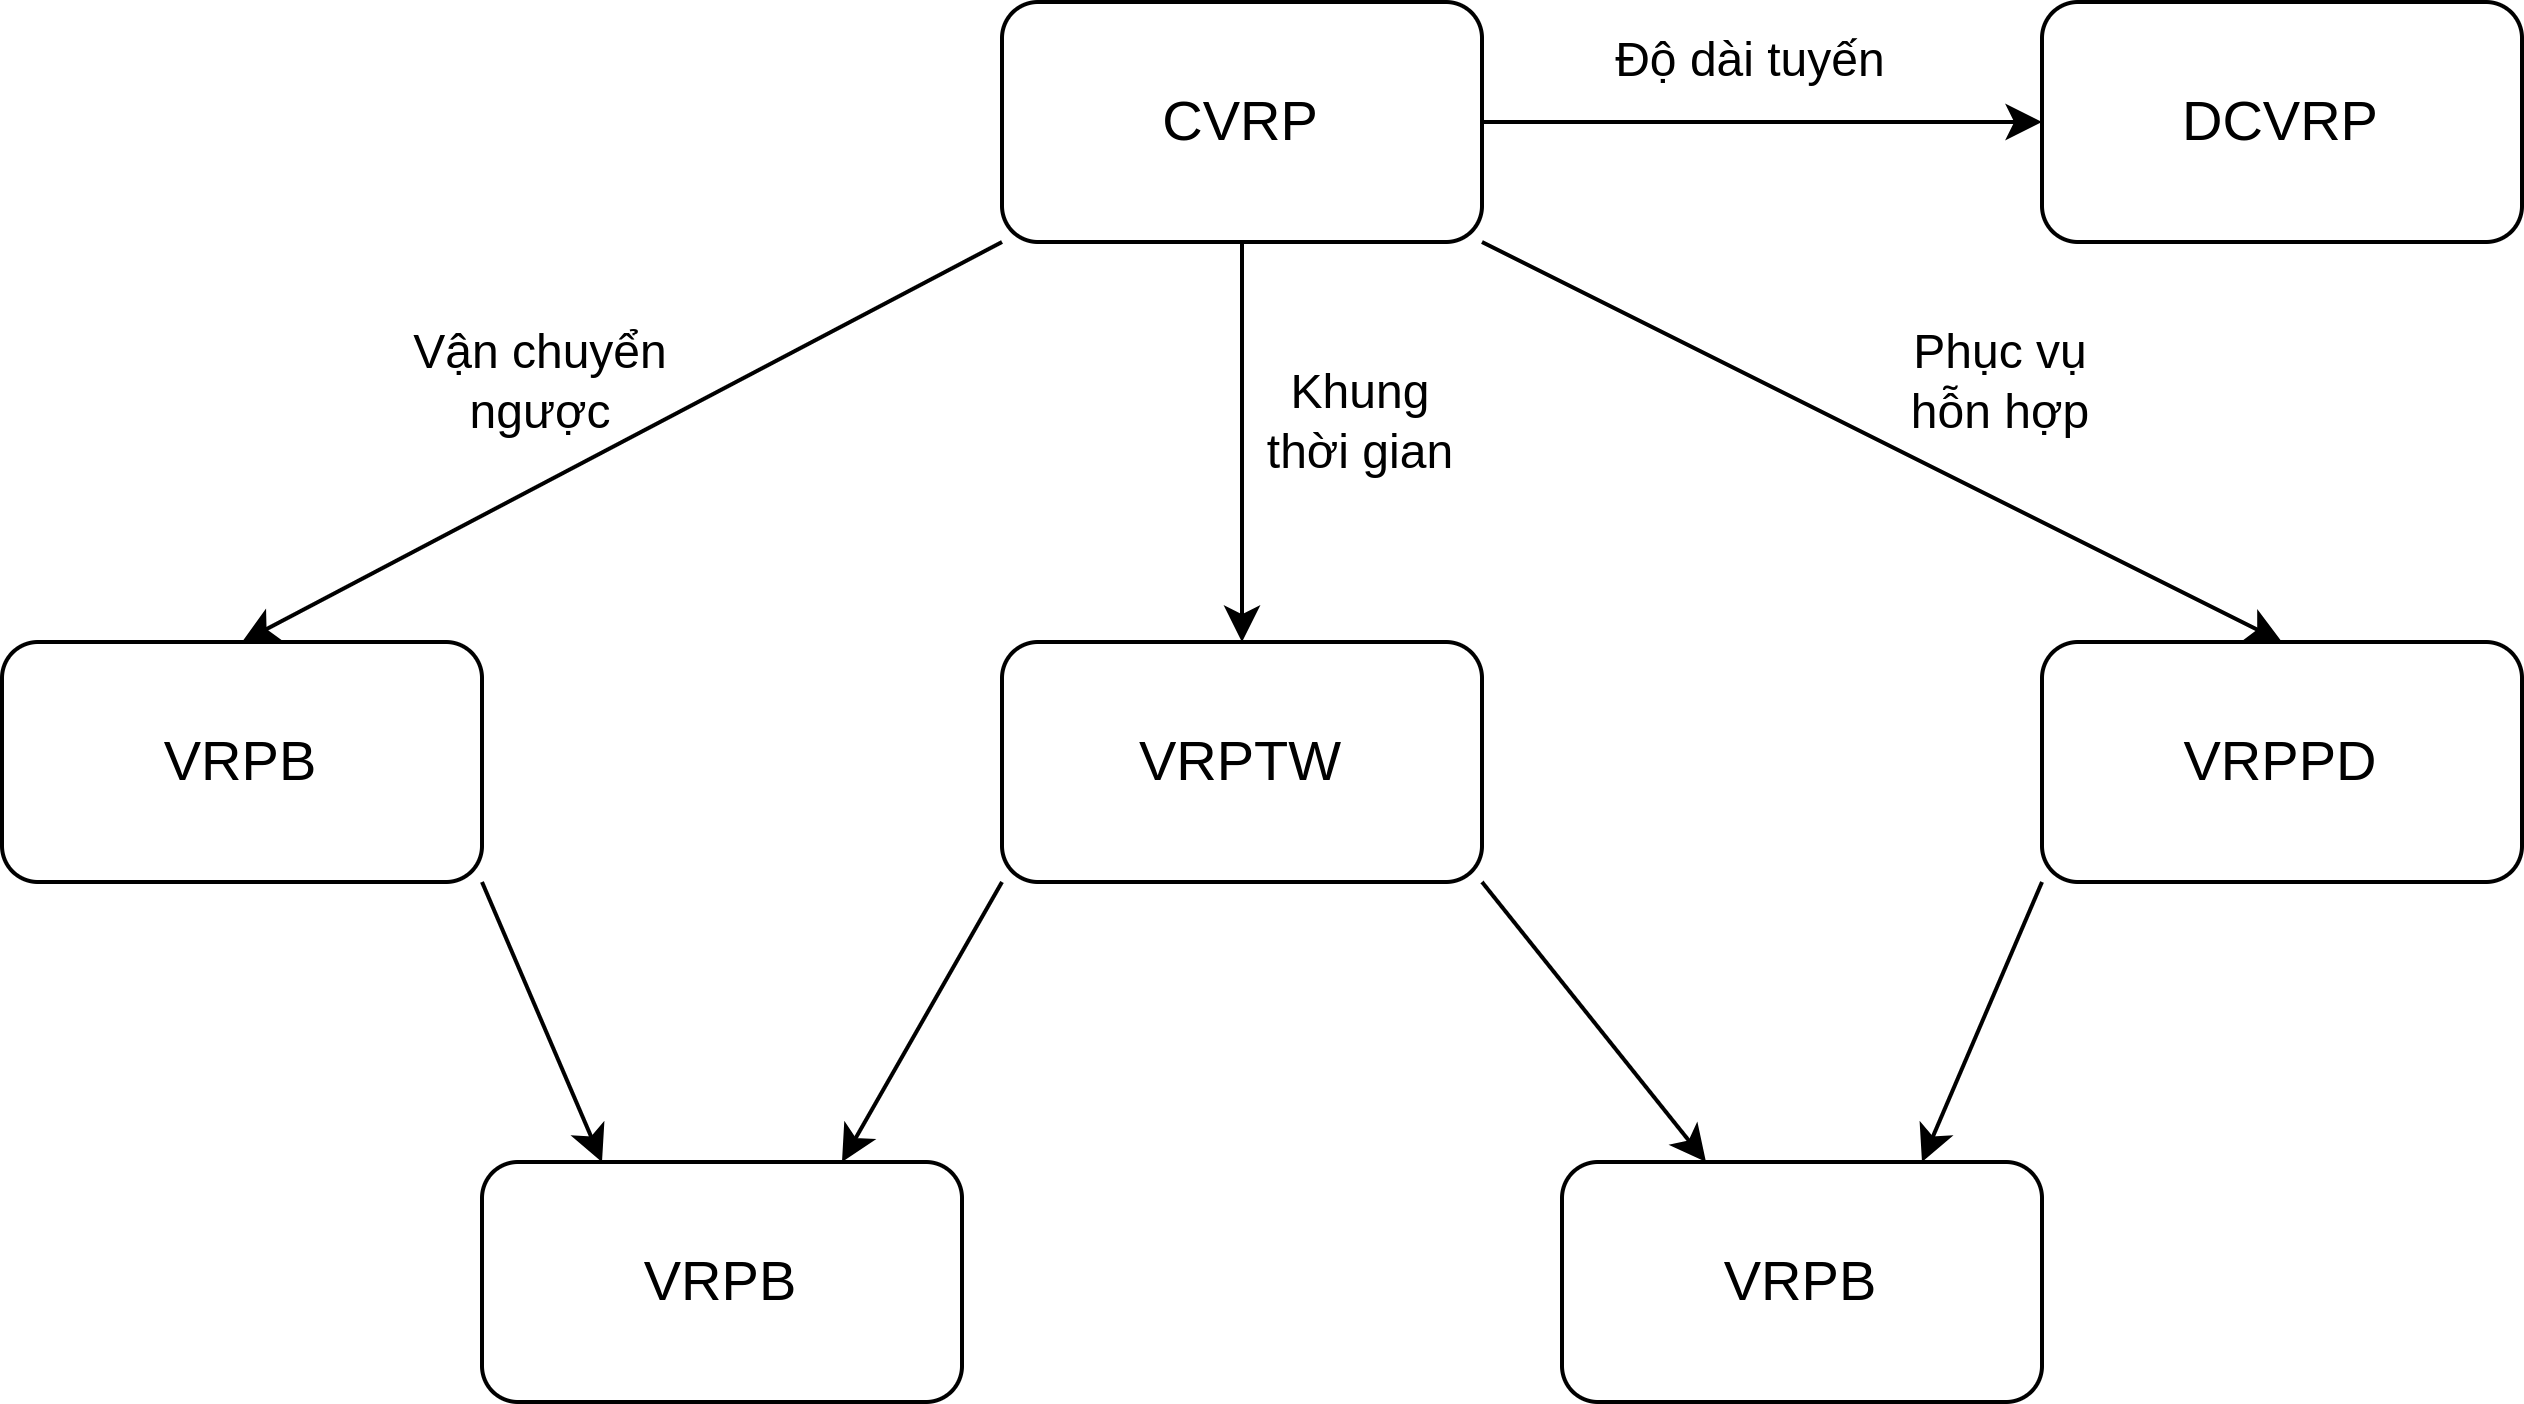
\includegraphics[width=0.8\textwidth]{figures/vrp.png} 
  \caption{Các bài toán, biến thể của VRP} % Creates caption underneath graph
  \label{fig:fg_01}
\end{figure}

\section{Định nghĩa bài toán}
\label{sec:def}

\subsection{CVRP}

Trước hết ta xem xét mô hình cho bài toán \textit{nguyên bản}: \textit{bài toán định tuyến xe với ràng buộc tải trọng}. Bài toán nguyên bản là CVRP mà không phải là VRP (không ràng buộc). Ta thấy rằng nếu không có bất kì ràng buộc nào thì một xe có thể phục vụ tất cả các yêu cầu và bài toán VRP sẽ trở thành TSP (\textit{travelling salesman problem}). Ít nhất ràng buộc về tải trọng là thực tế và giữ cho mỗi xe chỉ phục vụ được một số yêu cầu nhất định (trong trường hợp số yêu cầu không quá nhỏ cũng như tải trọng của xe là quá lớn).


Gọi $G=(V,A)$ là một độ thị đầy đủ với $V=\{ 0, ..., n \}$ là tập nút và $A$ là tập các cung. Các nút $i=1,...,n$ đại diện cho các yêu cầu hay khách hàng cần phục vụ, nút $0$ là kho hàng. Đôi khi, kho hàng cũng được biểu diễn bằng nút $n+1$.

Một số không âm được gọi là chi phí $c_{ij}$ đại diện cho mỗi cung $(i,j) \in A$. Nói cách khác, $c_{ij}$ là chi phí cần bỏ ra để di chuyển từ nút $i$ tới nút $j$. Trong bài toán này và hầu hết các bài toán định tuyến, ta không định nghĩa cạnh $(i,i)$ nên có thể gán $c_{ii} = \infty$ với $i \in V$.

Nếu đồ thị là có hướng thì ma trận chi phí $c$ là bất đối xứng, khi đó ta có bài toán CVRP bất đối xứng ACVRP (\textit{asymetric CVRP}). Ngược lại, nếu $c_{ij} = c_{ji}$ với mọi $(i,j) \in A$ ta có bài toán CVRP đối xứng SCVRP (\textit{symetric CVRP}) và các cung của $A$ được thay thế bằng tập cách cạnh vô hướng $E$. Với một cạnh $e \in E$, ta gọi $\alpha(e)$ và $\beta(e)$ là nút bắt đầu và kết thúc của cạnh.

Đồ thị $G$ phải là đồ thị liên thông và nhìn chung ta giả thiết đồ thị $G$ là đầy đủ. Với một nút $i$, gọi $\Delta^+(i)$ là tập ra của $i$ (\textit{forward star}), được định nghĩa là tập các nút $j$ mà cung $(i,j) \in A$, nói cách khác, đây là tập các nút có thể tiếp cận trực tiếp từ nút $i$. Tương tự như vậy, $\Delta^-{i}$ là tập vào của $i$ (\textit{backward star}), được định nghĩa là tập các nút $j$ mà cung $(j,i) \in A$ hay là tập các nút tiếp cận trực tiếp tới nút $i$. Với một tập nút con $S \subseteq V$, gọi $\delta(S)$ là tập các cạnh $e \in E$ chỉ có một hoặc cả hai đầu mút thuộc $S$. Để thuận tiện, khi xét một nút $i \in V$, ta viết $\delta(i)$ thay cho $\delta(\{i\})$.

Trong hầu hết các bài toán thực tế, ma trận chi phí thỏa mãn bất đẳng thức tam giác
\begin{equation}
	c_{ij} + c_{jk} \geq c_{ik}, \quad \forall i,j,k \in V.
\end{equation}
Nói cách khác, việc đi trực tiếp từ nút $i$ tới nút $j$ luôn tốn ít chi phí hơn là đi gián tiếp. Với nhiều thuật toán, bất đẳng thức tam giác là điều kiện cần, điều này có thể được đảm bảo bằng cách thêm một đại lượng dương lớn (hợp lý) vào chi phí của mỗi cung. Ta chú ý thêm rằng, nếu chi phí của mỗi cung thuộc đồ thị bằng với chi phí của đường đi ngắn nhất giữa hai đầu mút của cung thì mà trận chi phí thỏa mãn bất đẳng thức tam giác.

Trong nhiều trường hợp, tập các nút nằm trên một mặt phẳng, vị trí của chúng được cho bởi tọa độ và chi phí $c_{ij}$ của mỗi cung $(i,j) \in A$ là khoảng cách Euclide giữa hai điểm ứng với nút $i$ và $j$. Khi đó, ma trận chi phí là đối xứng và thỏa mãn bất đẳng thức tam giác. Bài toán này được gọi là \textit{Euclidian} SCVRP.

Mỗi khách hàng $i$ có một nhu cầu (về tải trọng) là $d_i$ và nhu cầu của kho $d_0=0$. Với một tập nút $S \subseteq V$, ta kí hiệu $d(S) = \sum_{i \in S} d_i$ là tổng nhu cầu của tập.

Một tập hợp $K$ đại diện cho các xe, mỗi xe có tải trọng $C$, các xe sẵn sàng ở kho tại thời điểm bắt đầu. Ta giả thiết $d_i \leq C$ với mỗi $i=1,...,n$. Điều kiện này này là cần thiết để  mỗi khách hàng đều được phục vụ. Mỗi xe phục vụ nhiều nhất một tuyến và ta giả thiết $K$ không nhỏ hơn $K_{min}$ với $K_{min}$ là số xe ít nhất cần để phục vụ toàn bộ khách hàng.

Với một tập $S \subseteq V \setminus \{0\}$, ta gọi $r(S)$ là số xe ít nhất để phục vụ toàn bộ khách hàng thuộc tập $S$. Chú ý rằng $r(V \setminus \{0\}) = K_{min}$.

CVRP yêu cầu tìm một tập chính xác $K$ các chu trình đơn (mỗi chu trình ứng với một tuyến đường) với tổng chi phí của tất cả các cung thuộc các chu trình này là nhỏ nhất. Lời giải phải thỏa mãn các ràng buộc sau
\begin{itemize}
	\item[] (i) mỗi chu trình đều đi qua nút ứng với kho hàng;
	\item[] (ii) mỗi nút ứng với một khách hàng được đi qua bởi đúng một chu trình;
	\item[] (iii) tổng nhu cầu của các khách hàng trong mỗi chu trình không được vượt quá tải trọng của xe.
\end{itemize}

\subsection{VRPTW}
Bài toán định tuyến xe với ràng buộc thời gian - VRPTW (\textit{VRP with time windows}) là một mở rộng của CVRP. Trong đó, ngoài ràng buộc về tải trọng cho mỗi xe, mỗi khách hàng $i$ bị ràng buộc bởi một khoảng thời gian $[a_i, b_i]$ được gọi là khung thời gian hay cửa sổ thời gian (\textit{time window}). Thời gian phục vụ khách hàng $i$ là $s_i$. Thời gian di chuyển từ nút $i$ tới nút $j$ là $t_{ij}$ với mỗi cung $(i,j) \in A$ hay $t_e$ với $e \in E$. Ngoài ra nếu xe đến nút $i$ sớm thì phải chờ đến thời gian $a_i$ mới được phục vụ. Nếu xe đến nút $i$ muộn hơn $b_i$ thì khách hàng sẽ không được phục vụ.

Thường thì ma trận chi phí và ma trận thời gian di chuyển là như nhau, hơn nữa các xe được giả thiết đều xuất phát từ kho tại thời điểm $0$. Ràng buộc thời gian dẫn tới việc mỗi tuyến đường là có hướng (có thứ tự đi đến các nút) ngay cả khi ma trận chi phí là đối xứng. Chính vì thế, VRPTW thường được mô tả như một bài toán bất đối xứng.

VRPTW yêu cầu tìm một tập chính xác $K$ chu trình đơn với tổng chi phí là nhỏ nhất, thỏa mãn các ràng buộc sau đây
\begin{itemize}
	\item[] (i) mỗi chu trình đều đi qua nút ứng với kho hàng;
	\item[] (ii) mỗi nút ứng với một khách hàng được đi qua bởi đúng một chu trình;
	\item[] (iii) tổng nhu cầu của các khách hàng trong mỗi chu trình không được vượt quá tải trọng của xe;
	\item[] (iv) với mỗi khách hàng $i$, thời gian bắt đầu phục vụ phải nằm trong khung thời gian $[a_i, b_i]$ và xe hoàn thành việc phục vụ sau khoảng thời gian $s_i$.
\end{itemize}

VRPTW là bài toán NP-khó, nó là trường hợp tổng quát của CVRP. Nếu ta đặt $a_i=0$ và $b_i=\infty$ với $i \in V \setminus \{0\}$ thì VRPTW trở thành CVRP. Ngoài ra ta cũng thu được biến thể TSP với ràng buộc thời gian (TSPTW) nếu $C \geq d(V)$ và $K=1$.

\subsection{VRPPD}
Một biến thể khác nữa của CVRP là bài toán định tuyến xe với lấy và giao hàng (\textit{VRP with pickup and delivery - VRPPD}). Trong đó, mỗi khách hàng $i$ có thêm hai đại lượng đặc trưng nữa là $d_i$ và $p_i$ lần lượt là nhu cầu lấy và giao (của khách hàng) tại vị trí của khách hàng $i$. Đôi khi, ta chỉ dùng một đại lượng $d_i = d_i - p_i$ cho mỗi khách hàng $i$ để chỉ lượng nhu cầu chênh lệch giữa việc lấy và giao hàng (có thể là số âm). Với mỗi khách hàng $i$, gọi $O_i$ là nút đại diện cho điểm giao hàng và $D_i$ là nút đại diện cho điểm lấy hàng.

Với mỗi khách hàng, ta giả thiết điểm giao được phục vụ trước điểm lấy. Do đó, tải hiện tại của một xe trướ khi tới điểm đã cho là tải ban đầu trừ đi tổng nhu cầu đã giao cộng với tổng nhu cầu đã lấy.

VRPPD yêu cầu tìm chính xác một tập $K$ các chu trình đơn với tổng chi phí là nhỏ nhất, thỏa mãn các ràng buộc sau đây

\begin{itemize}
	\item[] (i) mỗi chu trình đều đi qua nút ứng với kho hàng;
	\item[] (ii) mỗi nút ứng với một khách hàng được đi qua bởi đúng một chu trình;
	\item[] (iii) tải hiện tại của xe trong suốt quá trình phục vụ không âm và không được vượt quá tải trọng của xe;
	\item[] (iv) với mỗi khách hàng $i$, khách hàng $O_i$ khác với kho phải được phục vụ trong cùng một tuyến và trước khách hàng $i$;
	\item[] (v) với mỗi khách hàng $i$, khách hàng $D_i$ khác với kho phải được phụ vụ trong cùng một tuyến và sau khách hàng $i$.
\end{itemize}

VRPPD là trường hợp tổng quát của CVRP. Nếu ta đặt $O_i = D_i = 0$ và $p_i = 0$ cho mọi $i \in V$ thì VRPPD suy biến về CVRP. Hơn nữa nếu đặt $K=1$ thì ta thu được TSP với lấy và giao hàng (\textit{TSP with pickup and delivery - TSPPD}).

\section{Mô hình toán học}
\label{sec:math}

Phần tiếp theo, ta trình bày một số mô hình toán học cơ bản cho VRP theo P. Toth và D. Vigo \cite{toth2002vehicle}. Mô hình cụ thể cho VRPTW được trình bày ở phần \ref{sec:math_vrptw}. 

\subsection{Các mô hình cơ bản cho VRP}
\label{sec:math_common}

Trong phần này, chúng ta cùng xem xét các mô hình toán học cơ bản cho VRP và xem xét cách các mô hình này được mở rộng để kết hợp hay bổ sung ràng buộc hoặc hàm mục tiêu.

Có ba cách tiếp cận để mô hình hóa VRP. Loại mô hình đầu tiên là "công thức dòng xe" (\textit{vehicle flow formulations}) sử dụng các biến nguyên ứng với mỗi cung hay cạnh của đồ thị. Các biến này để đếm số lần mà xe đi qua cung hay cạnh đó. Loại mô hình này thường được sử dụng cho những phiên bản cơ bản của VRP. Mô hình đặc biệt phù hợp cho những trường hợp mà tổng chi phí, hay hàm mục tiêu có thể biểu diễn bằng tổng chi phí của mỗi cung hay cạnh và hầu hết các ràng buộc liên quan đến sự thay đổi giữa các yêu cầu trong cùng một tuyến. Khi đó, mô hình có thể được xây dựng một cách hiệu quả qua việc định nghĩa hợp lý tập cung và chi phí của cung. Tuy nhiên, "công thức dòng xe" không được sử dụng cho các bài toán mà tổng chi phí phụ thuộc vào chuỗi (có thứ tự) các nút hoặc phụ thuộc vào loại phương tiện.

Loại mô hình thứ hai là "công thức dòng hàng" (\textit{commodity flow formulation}). Trong loại mô hình này, các biến nguyên ứng với mỗi cung hoặc cạnh biểu diễn "dòng" của lượng hàng dọc theo các tuyến đường. "Công thức dòng hàng" thường được sử dụng làm cơ sở cho các phương pháp giải chính xác VRP.

Loại mô hình cuối cùng có số biến nhị phân tăng theo cấp số nhân với kích thước của đầu vào, mỗi biến biểu thị cho một chu trình khả thi khác nhau. Trong loại mô hình này, VRP được mô hình hóa như một bài toán phân hoạch tập hợp (\textit{Set-Partitioning Problem - SPP}). SSP xác định một tập các chu trình có chi phí nhỏ nhất phục vụ mỗi yêu càu một lần và thỏa mãn các ràng buộc. Ưu điểm chính của loại mô hình này là nó cho phép tổng quát hóa chi phí của các tuyến đường ví dụ như khi chi phí của tuyến phụ thuộc vào toàn bộ chuỗi các cung hay cạnh và phụ thuộc vào loại xe. Hơn nữa, các ràng buộc không cần tính đến tính khả thi của một tuyến đường đơn lẻ. Kết quả là ràng buộc có thể được thay thế bằng các bất đẳng thức gọn gàng hơn. Đánh đổi lại, loại mô hình này cần một số lượng biến biểu diễn rất lớn.

\subsubsection*{Mô hình dòng xe}

Trước tiên, chúng ta mô tả công thức "lập trình tuyến tính nguyên" (\textit{integer linear programming}) cho ACVRP, sau đó là SCVRP. Mô hình "công thức dòng xe hai chỉ số" (\textit{two-index vehicle flow formulation}) sử dụng $O(n^2)$ biến nhị phân $x$ để chỉ thị nếu một xe đi qua cung $(i,j)$ hay không. Nói cách khác, $x_{ij}$ nhận giá trị bằng $1$ nếu cung $(i, j) \in A$ nằm trong nghiệm tối ưu và $0$ nếu trong trường hợp còn lại. 

\begin{equation} \label{eq:vrp1}
  \text{(VRP1)} \quad \min \sum_{i \in V} \sum_{j \in V} c_{ij} x_{ij}
\end{equation}
s.t.
\begin{flalign}
	\label{ct_vrp1:1}  & \sum_{i \in V} x_{ij} = 1, \quad \forall j \in V \setminus \{0\}, \\
  \label{ct_vrp1:2}  & \sum_{j \in V} x_{ij} = 1, \quad \forall i \in V \setminus \{0\}, \\
  \label{ct_vrp1:3}  & \sum_{i \in V} x_{i0} = K, \\
  \label{ct_vrp1:4}  & \sum_{j \in V} x_{0j} = K, \\
  \label{ct_vrp1:5}  & \sum_{i \notin  S} \sum_{j \in S} x_{ij} \geq r(S), \quad \forall S \subseteq V \setminus \{0\}, S \neq \emptyset, \\
  \label{ct_vrp1:6}  & x_{ij} \in \{0,1\}, \quad \forall i,j \in V.
\end{flalign}
Ràng buộc (\ref{ct_vrp1:1}) và (\ref{ct_vrp1:2}) đảm bảo chỉ có đúng một cung vào và một cung ra cho mỗi nút ứng với mỗi yêu cầu. Ràng buộc (\ref{ct_vrp1:3}) và (\ref{ct_vrp1:4}) đảm bảo có đúng $K$ xe xuất phát từ kho và trở về kho. Ràng buộc (\ref{ct_vrp1:5}) đảm bảo số xe được sử dụng không nhỏ hơn số xe tối thiểu cần để phục vụ tất cả các yêu cầu. Trong thực tế, nhiều khi ràng buộc này được phát biểu lại là tổng số xe sử dụng không vượt quá một giới hạn trên $K_{max}$ nhất định. 

Đối với hệ đối xứng, \textit{VRP1} được viết lại như sau

\begin{equation} \label{eq:vrp2}
	\text{(VRP2)} \quad \min \sum_{i \in V \setminus \{n\}} \sum_{j > i} c_{ij} x_{ij}
\end{equation}
s.t.
\begin{flalign}
	\label{ct_vrp2:1}  & \sum_{h < i} x_{hi} + \sum_{j < i} x_{ij} = 2, \quad \forall j \in V \setminus \{0\}, \\
  \label{ct_vrp2:2}  & \sum_{j \in V \setminus \{0\}} x_{0j} = 2K, \\
  \label{ct_vrp2:3}  & \sum_{i \in S} \sum_{h < i, h \notin S} x_{hi} + \sum_{i \in S} \sum_{j < i, j \notin S} x_{ij} \geq 2r(S), \quad \forall S \subseteq V \setminus \{0\}, S \neq \emptyset, \\
  \label{ct_vrp2:4}  & x_{ij} \in \{0,1\}, \quad \forall i,j \in V \setminus \{0\}, i < j, \\
  \label{ct_vrp2:5}  & x_{0j} = \{0, 1, 2\}, \quad \forall i \in V \setminus \{0\}.
\end{flalign}
Ràng buộc (\ref{ct_vrp2:1}) và (\ref{ct_vrp2:2}) đảm bảo chỉ có đúng một cung vào và một cung ra cho mỗi nút ứng với mỗi yêu cầu, $2K$ để đảm bảo số xe xuất phát và kết thúc tại kho. Ràng buộc (\ref{ct_vrp2:3}) đảm bảo số xe được sử dụng không nhỏ hơn số xe tối thiểu cần để phục vụ tất cả các yêu cầu. 

Phiên bản mô hình 2 chỉ số cho trường hợp hệ đối xứng có thể được biểu diễn chỉ với một chỉ số $e$ biểu thị cho cạnh vô hướng $e \in E$. Nếu ta không cho phép tuyến chỉ chứa đúng một yêu cầu thì các biến sử dụng đều là nhị phân. Ngoài ra, nếu $e \notin \delta(0)$ thì $x_e \in \{0, 1\}$ và nếu $e \in \delta(0)$ thì $x_e \in \{0, 1, 2\}$. Công thức \textit{VRP2} được viết lại như sau

\begin{equation} \label{eq:vrp3}
	\text{(VRP3)} \quad \min \sum_{e \in E} c_e x_e
\end{equation}
s.t.
\begin{flalign}
	\label{ct_vrp3:1}  & \sum_{e \in \delta(i)} x_e = 2, \quad \forall i \in V \setminus \{0\}, \\
  \label{ct_vrp3:2}  & \sum_{e \in \delta(0)} x_e = 2K, \\
  \label{ct_vrp3:3}  & \sum_{e \in \delta(S)} x_e \geq 2r(S), \quad \forall S \subseteq V \setminus \{0\}, S \neq \emptyset, \\
  \label{ct_vrp3:4}  & x_e \in \{0,1\}, \quad \forall e \notin \delta(0), \\
  \label{ct_vrp3:5}  & x_e \in \{0,1,2\}, \quad \forall e \in \delta(0).
\end{flalign}

Mô hình dòng xe hai chỉ số được sử dụng khá rộng rãi trong các biến thể cơ bản của SCVRP và ACVRP chẳng hạn như VRPB. Tuy nhiên, mô hình này là không đủ mạnh cho các biến thể phức tạp hơn ví dụ như khi tổng chi phí phụ thuộc vào một chuỗi (có thứ tự) các nút hoặc phụ thuộc vào loại phương tiện. Ngoài ra, ta cũng không biết một cách tường minh xe nào được dùng cho tuyến đường. 

Một mô hình mở rộng để khắc phục các điểm yếu của mô hình dòng xe hai chỉ số là mô hình dòng xe ba chỉ số (\textit{three-index vehicle flow formulation}). Mô hình này sử dụng $O(n^2K)$ biến nhị phân $x$. Biến $x_{ijk}$ đếm số lần cung $(i, j) \in A$ được đi qua bởi xe $k$ với $k=1,...,K$ trong nghiệm tối ưu. Ngoài ra ta sử dụng thêm $O(nK)$ biến nhị phân $y$, với $y_{ik}$ ($i \in V; k=1,...,K$) nhận giá trị $1$ nếu yêu cầu $i$ được phục vụ bởi xe $k$ và $0$ trong trường hợp còn lại. Mô hình ba chỉ số cho ACVRP được mô tả như sau

\begin{equation} \label{eq:vrp4}
	\text{(VRP4)} \quad \min \sum_{i \in V} \sum_{j \in V} c_{ij} \sum_{k=1}^K x_{ijk}
\end{equation}
s.t.
\begin{flalign}
	\label{ct_vrp4:1}  & \sum_{k=1}^K y_{ik} = 1, \quad \forall i \in V \setminus \{0\}, \\
  \label{ct_vrp4:2}  & \sum_{k=1}^K y_{0k} = K, \\
  \label{ct_vrp4:3}  & \sum_{j \in V} x_{ijk} = \sum_{j \in V} x_{jik} = y_{ik}, \quad \forall i \in V \setminus \{0\}, k=1,...,K, \\
  \label{ct_vrp4:4}  & \sum_{i \in V} d_i y_{ik} \leq C, \quad \forall k=1,...,K, \\
  \label{ct_vrp4:5}  & \sum_{i \in S} \sum_{j \notin S} x_{ijk} \geq y_{hk}, \quad \forall S \subseteq V \setminus \{0\}, h \in S, k=1,...,K, \\
  \label{ct_vrp4:6}  & y_{ik} \in \{0,1\}, \quad \forall i \in V, k=1,...,K, \\
  \label{ct_vrp4:7}  & x_{ijk} \in \{0,1\}, \quad \forall i,j \in V, k=1,...,K.
\end{flalign}
Ràng buộc (\ref{ct_vrp4:1}) đảm bảo mỗi yêu cầu được phục vụ đúng một lần. Ràng buộc (\ref{ct_vrp4:2}) đảm bảo có $K$ xe xuất phát từ kho. Ràng buộc (\ref{ct_vrp4:3}) đảm bảo có cùng số xe đến và rời khỏi vị trí của mỗi yêu cầu. Ràng buộc (\ref{ct_vrp4:4}) là ràng buộc về tải trọng của xe. Ràng buộc (\ref{ct_vrp4:5}) đảm bảo tính kết nối trong tuyến đường được phục vụ bởi xe $k$.

Đối với bài toán đối xứng, ta có phiên bản hai chỉ số cho mô hình trên với biến nhị phân $x_{ek}$, $e \in E$ và $k=1,...,K$

\begin{equation} \label{eq:vrp5}
	\text{(VRP5)} \quad \min \sum_{e \in E} c_{ij} \sum_{k=1}^K x_{ek}
\end{equation}
s.t.
\begin{flalign}
	\label{ct_vrp5:1}  & \sum_{k=1}^K y_{ik} = 1, \quad \forall i \in V \setminus \{0\}, \\
  \label{ct_vrp5:2}  & \sum_{k=1}^K y_{0k} = K, \\
  \label{ct_vrp5:3}  & \sum_{e \in \delta(i)} x_{ek} = 2y_{ik}, \quad \forall i \in V, k=1,...,K, \\
  \label{ct_vrp5:4}  & \sum_{i \in V} d_i y_{ik} \leq C, \quad \forall k=1,...,K, \\
  \label{ct_vrp5:5}  & \sum_{e \in \delta(S)} x_{ijk} \geq 2y_{hk}, \quad \forall S \subseteq V \setminus \{0\}, h \in S, k=1,...,K, \\
  \label{ct_vrp5:6}  & y_{ik} \in \{0,1\}, \quad \forall i \in V, k=1,...,K, \\
  \label{ct_vrp5:7}  & x_{ek} \in \{0,1\}, \quad \forall e \notin \delta(0), k=1,...,K, \\
  \label{ct_vrp5:8}  & x_{ek} \in \{0,1,2\}, \quad \forall e \in \delta(0), k=1,...,K.
\end{flalign}

Công thức dòng xe ba chỉ số được sử dụng cho các biến thể  VRP với nhiều ràng buộc ví dụ như VRPTW. Công thức này được trình bày trong phần \ref{sec:math_vrptw}. Công thức dòng hàng và công thức phân hoạch tập hợp được trình bày trong chương \ref{chap:solution}.

\subsection{Mô hình cho biến thể VRPTW}
\label{sec:math_vrptw}

Trong phần này, ta trình bày biểu diễn toán học cho bài toán VRPTW. Trong khuôn khổ luận văn này, tác giả tập trung thực nghiệm giải quyết VRPTW, từ đó ta cũng có thể giản ước về CVRP cũng như tổng quát với VRPPD (\textit{VRP with pickup and delevery}) hoặc PDPTW (\textit{pickup and delivery with time window}). Như đã trình bày ở phần trước, VRPTW là một mở rộng của CVRP với ràng buộc khung thời gian. Trong đó, mỗi khách hàng $i$ được ràng buộc bởi một khung thời gian $[a_i,b_i]$. Xe không được đến $i$ tại thời điểm $t_i > b_i$, ngoài ra, nếu đến sớm hơn thởi điểm $a_i$ hay $t_i < a_i$ thì xe cần phải chờ tới thời điểm $a_i$ để phục vụ khách hàng. Thời gian phục vụ của khách hàng $i$ là $s_i$.

VRPTW là bài toán NP-khó, việc tìm lời giải hay nghiệm tối ưu (chính xác) gần như là bất khả thi với các bài toán có kích thước đầu vào lớn. Để dễ hình dung, xét bài toán VRP, với số lượng khách hàng $n=100$, và chỉ một xe, số lượng lời giải là $n! \approx 10^{158}$. Nếu ta có số CPU ước tính bằng toàn bộ số nguyên tử trong vũ trụ $n_{CPU} \approx 10^{80}$, thời gian nhỏ nhất là thời gian Plank $t_p \approx 5.39 \times 10^{-44}$. Để kiểm tra toàn bộ lời giải có phải nghiệm tối ưu ta cần thời gian $T \approx 10^{158} \times 5.39 \times 10^{-44} / 10^{80} \approx 5.39 \times 10^{34}$. Để so sánh, tuổi của vũ trụ được ước tính khoảng $4.33 \times 10^{17}$. Nghĩa là ta sẽ mất thời gian lớn gấp cỡ \textit{một trăm triệu tỉ} lần tuổi của cả vũ trụ! \footnote[1]{Slides của Thibaut Vidal (SOICT, Nha Trang 2017)}

Như đã trình bày ở phần \ref{sec:def}, VRPTW được định nghĩa trên đồ thị $G = (V, A)$, kho hàng được biểu diễn bởi nút $0$ và $n+1$. Một tuyến thỏa mãn là một đường đi trên đồ thị $G$ bắt đầu từ $0$ và kết thúc ở $n+1$. Nếu kho hàng được biểu diễn chỉ bởi nút $0$ thì tuyến thỏa mãn là một đơn chu trình trên đồ thị $G$ chứa nút $0$. Khung thời gian của nút $0$ và $n+1$ là $[a_0, b_0] = [a_{n+1}, b_{n+1}] = [E, L]$, trong đó $E$ và $L$ lần lượt là thời gian sớm nhất rời kho và thời gian muộn nhất trở về kho. Ngoài ra, thời gian phục vụ và nhu cầu của kho đều được đặt bằng 0, hay $s_0 = s_{n+1} = 0$ và $d_0 = d_{n+1} = 0$. Lời giải chấp nhận được chỉ tồn tại nếu $a_0 = E \leq \min_{i \in V \setminus \{0\}} \{b_i - t_{0i}\}$ và $b_{n+1} = L \geq \min_{i \in V \setminus \{0\}} \{ a_i + s_i + t_{0i} \}$. Chú ý rằng, cung $(i,j) \in A$ có thể được bỏ đi nếu không thỏa mãn ràng buộc thời gian $a_i + s_i + t_{ij} > b_j$ hoặc vi phạm ràng buộc về tải trọng $d_i + d_j > C$. Cuối cùng, nếu mục tiêu chính là giảm thiểu số lượng xe thì cung $(0,n+1)$ với $c_{0,n+1} = t_{0,n+1} = 0$ phải được thêm vào $A$.

Tiếp theo, chúng ta trình bày một mô hình toán cho VRPTW với hai biến: biến $x_{ijk}$ (\textit{flow variable}) với $(i,j) \in A, k \in K$ nhận giá trị 1 nếu xe $k$ đi trực tiếp từ nút $i$ tới nút $j$ và 0 nếu ngược lại. Biến $w_{ik}$ với $i \in V, k \in K$ là thời gian bắt đầu phục vụ khách hàng $i$ bởi xe $k$. VRPTW được mô hình một cách chính tắc như sau theo Toth (2002) \cite{toth2002vehicle}

\begin{equation} \label{eq1}
	\min \sum_{k \in K} \sum_{(i,j) \in A} c_{ij} x_{ijk}
\end{equation}
s.t.
\begin{flalign}
	\label{ct:1}  & \sum_{k \in K} \sum_{j \in \Delta^+(i)} x_{ijk} = 1, \quad \forall i \in N, \\
	\label{ct:2}  & \sum_{j \in \Delta^+(0)} x_{0jk} = 1, \quad \forall k \in K,                   \\
	\label{ct:3}  & \sum_{i \in \Delta^-(j)} x_{ijk} -  \sum_{i \in \Delta^+(j)} x_{jik} = 0, \quad \forall k \in K, j \in N, \\
	\label{ct:4}  & \sum_{i \in \Delta^-(n+1)} x_{i,n+1,k} = 1, \quad \forall k \in K, \\
	\label{ct:5}  & x_{ijk} (w_{ik} + s_i + t_{ij} - w_{jk}) \leq 0, \quad \forall k \in K, (i,j) \in A, \\
	\label{ct:6}  & a_i \sum_{j \in \Delta^+(i)} x_{ijk} \leq w_{ik} \leq b_i \sum_{j \in \Delta^+(i)} x_{ijk}, \quad \forall k \in K, i \in N, \\
	\label{ct:7}  & E \leq w_{ik} \leq L, \quad \forall k \in K, i \in \{0, n+1\}, \\
	\label{ct:8}  & \sum_{i \in N} d_i \sum_{j \in \Delta^+(i)} x_{ijk} \leq C, \quad \forall k \in K, \\
	\label{ct:9}  & x_{ijk} \geq 0, \quad \forall k \in K, (i,j) \in A, \\
	\label{ct:10} & x_{ijk} \in \{0,1\}, \quad \forall k \in K, (i,j) \in A.
\end{flalign}
Hàm mục tiêu trong phương trình (\ref{eq1}) biểu diễn tổng chi phí của tất cả các tuyến đường.
Tập $N = V \setminus \{0\}$ biểu diễn cho tập khách hàng.

\begin{itemize}
	\item Ràng buộc (\ref{ct:1}) đảm bảo rằng mỗi khách hàng chỉ được phục vụ bởi một xe.
	\item Ràng buộc (\ref{ct:2}) đảm bảo rằng mỗi xe phải xuất phát từ kho hàng.
	\item Ràng buộc (\ref{ct:3}) đảm bảo rằng trên một tuyến, nếu khách hàng $i$ được phục vụ thì trước và sau đó đều có một khách hàng khác được phục vụ hoặc trước và sau đó là kho hàng. Nói cách khác, khách hàng $i$ phải ở giữa tuyến.
	\item Ràng buộc (\ref{ct:4}) đảm bảo rằng mỗi xe phải trở về kho hàng.
	\item Ràng buộc (\ref{ct:5}) đảm bảo về khung thời gian khi xe đi từ khách hàng $i$ tới khách hàng $j$. Nếu xe $k$ đi từ khách hàng $i$ tới khách hàng $j$ thì thời gian bắt đầu phục vụ khách hàng $i$ cộng với thời gian phục vụ khách hàng $i$ cộng với thời gian di chuyển từ khách hàng $i$ tới khách hàng $j$ phải nhỏ hơn hoặc bằng thời gian bắt đầu phục vụ khách hàng $j$. Dấu bằng xảy ra khi xe đến $j$ sau thời điểm $a_j$ (khách hàng $j$ được phục vụ luôn), nếu đến sớm hơn thì xe phải chờ để phục vụ khách hàng.
	\item Ràng buộc (\ref{ct:6}) đảm bảo rằng thời gian bắt đầu phục vụ khách hàng $i$ bởi xe $k$ nằm trong khung thời gian $[a_i, b_i]$.
	\item Ràng buộc (\ref{ct:7}) đảm bảo rằng thời gian bắt đầu phục vụ khách hàng $i$ bất kì phải nằm trong khoảng thời gian từ sớm nhất xuất phát từ kho và muộn nhất về kho.
	\item Ràng buộc (\ref{ct:8}) đảm bảo rằng tổng tải của mỗi xe không được vượt quá tải trọng tối đa $C$.
	\item Ràng buộc (\ref{ct:9}) và (\ref{ct:10}) đảm bảo điều kiện nhị phân của \textit{flow variable} $x_{ijk}$.
\end{itemize}

Ta có thể nhận thấy rằng, ràng buộc (\ref{ct:6}) ép $w_{ik} = 0$ nếu như khách hàng $i$ không được phục vụ bởi xe $k$. Điều kiện nhị phân trong ràng buộc (\ref{ct:10}) cho phép ràng buộc (\ref{ct:5}) được thay thế bởi
\begin{equation}
	\label{ct:5'}
	w_{ik} + s_i + t_{ij} - w_{jk} \leq (1 - x_{ijk}) M_{ij}, \quad \forall k \in K, (i,j) \in A,
\end{equation}
với $M_{ij}$ là các hằng số rất lớn. Hơn nữa $M_{ij}$ có thể thay bằng $\max \{b_i + s_i + t_{ij} - a_j, 0\}$ với $(i,j) \in A$ và như vậy ta chỉ cần kiểm tra ràng buộc (\ref{ct:5}) và (\ref{ct:5'}) cho các cung $(i, j) \in A$ thỏa mãn $M_{ij} > 0$. Mặt khác, khi $\max \{b_i + s_i + t_{ij} - a_j, 0\} = 0$ các điều kiện này được thỏa mãn với mọi $w_{ik}$, $w_{jk}$ và $x_{ijk}$.

Chúng ta không cần đưa ra mô hình cho CVRP nữa, bởi ta có thể bỏ qua các ràng buộc về thời gian ở điều kiện từ (\ref{ct:5}) đến (\ref{ct:7}). Khi đó VRPTW sẽ trở thành CVRP như đã trình bày ở những phần trước đó. Tác giả cũng không đưa ra mô hình cho VRPPD hay PDPTW để tránh sự phức tạp. VRPTW vừa đủ để ta có một mô hình đẹp và thực tế.
        \chapter{Một số phương pháp cho VRP}
\label{chap:solution}

Trong chương này, chúng ta sẽ xem xét một số khái niệm cần thiết và phương pháp để giải (lớp) bài toán định tuyến xe. Trong suốt chặng đường hơn 60 năm của bài toán VRP, có rất nhiều phương pháp được nghiên cứu và thực nghiệm từ các thuật toán giải chính xác đến các thuật toán xấp xỉ. Ba lớp thuật toán được trình bày bao gồm \textit{thuật toán chính xác}, \textit{heuristics cổ điển} và \textit{metaheuristics}. Lớp các thuật toán được trình bày một cách khái quát theo G. Laporte \cite{laporte2009fifty}. Cuối cùng tác giả đưa ra lựa chọn và đi sâu vào thuật toán tìm kiếm lân cận rộng thích ứng - ALNS (\textit{Adaptive Large Neighborhood Search}) để giải quyết bài toán VRPTW trong luận văn này.

\section{Thuật toán chính xác}

\subsection{Nhánh và cận}

Một trong những thuật toán chính xác được nghiên cứu sớm nhất là \textit{nhánh và cận}, lần đầu xuất hiện trong bài báo \textit{"An Algorithm for the Vehicle Dispatching Problem"} của N. Christofides và S. Eilon năm 1969 \cite{christofides1969algorithm}. Với $m$ là tham số đầu vào, đầu tiên đồ thị được mở rộng với việc thêm vào $m-1$ kho ảo và đặt chi phí của chúng bằng một số vô cùng lớn. Sau đó giải bài toán m-TSP trên đồ thị này bằng thuật toán TSP được trình bày bởi Little et al. (1963) \cite{little1963algorithm}

Hiệu năng của các thuật toán nhánh-cận đầu tiên được cải thiện đáng kể hai phương pháp cận dưới là k-degree centre trees (k-DCT) và q-routes (Christofides et al. (1981) \cite{christofides1981exact}).

\subsection{Quy hoạch động}

Eilon, Watson-Gandy và Christofides (1971) \cite{christofides1969algorithm} đưa ra lời giải cho bài toán VRP bằng phương pháp quy hoạch động. Gọi $c(S)$ là chi phí tối ưu của một tuyến ứng với tập nút $S \subseteq V \setminus \{0\}$. Mục tiêu là cực tiểu hóa $\sum_{r=1}^{m} c(S_r)$ trên tất cả các quy hoạch khả dĩ $\{S_1,...,S_m\}$ của $V \setminus \{0\}$. Gọi $f_k(U)$ là chi phí nhỏ nhất có thể đạt được khi sử dụng $k$ xe cho một tập con $U$ của $V \setminus \{0\}$. Ta có
\begin{equation}
	\label{eq:dp}
	f_k(U) =
	\begin{cases}
		c(U) \quad \text{nếu } k = 1,                                                                                      \\
		\min_{U^* \subseteq U \subseteq V \setminus \{0\}} \{f_{k-1} (U \setminus U^*) + c(U^*)\} \quad \text{nếu } k > 1. \\
	\end{cases}
\end{equation}
Chi phí tối ưu là $f_m(V \setminus \{0\})$ và các tuyến là các phân hoạch của $V \setminus \{0\}$ theo phương trình (\ref{eq:dp}).

\subsection{Công thức dòng xe}
Công thức 2-chỉ số cho bài toán VRP được nghiên cứu đầu tiên bởi Laporte, Nobert (1983) \cite{laporte1983branch} và Laporte, Nobert, Desrochers (1985) \cite{laporte1985optimal} và mở rộng công thức TSP cổ điển của Dantzig, Fulkerson, Johnson (1954) \cite{dantzig1954solution}. Gọi $x_{ij}$ là biến 0-1-2 bằng số lần một xe đi qua cung $(i,j)$. Bài toán được mô hình hóa như sau
\begin{equation}
	\min \sum_{(i,j) \in E} c_{ij} x_{ij}
\end{equation}
s.t.
\begin{flalign}
	\label{ct2:1} & \sum_{j=1}^n x_{0j}=2m, & \quad \\
	\label{ct2:2} & \sum_{i<k} x_{ik} + \sum_{j>k} x_{kj} = 2 & \quad \forall k \in V \setminus \{0\}, \\
	\label{ct2:3} & \sum_{i,j \in S} x_{ij} \leq |S| - \nu(S) & \quad \forall S \subseteq V \setminus \{0\}, \\
	\label{ct3:3} & x_{0j} \in \{0,1,2\} & \quad \forall j \in V \setminus \{0\}, \\
	\label{ct2:4} & x_{ij} \in \{0,1\} & \quad \forall i,j \in V \setminus \{0\},
\end{flalign}
trong đó $\nu(S)$ là cận dưới của số lượng xe cần thiết để phục vụ tập $S$. Công thức dòng xe và các biến thể đã được trình bày kĩ từ chương \ref{chap:model}.

\subsection{Công thức dòng hàng}
Trong công thức dòng hàng, biến $y_{ij}$ (hoặc $y_{ijk}$) định nghĩa tải (lượng hàng) của xe mang theo trên cung $(i,j)$. Ví dụ được trình bày bởi Gavish, Graves (1979) \cite{gavish1978travelling}, tuy nhiên các tác giả không đưa ra kết quả tính toán. Các ví dụ gần đây hơn được nghiên cứu bởi Baldacci, Hadjiconstantinou, Mingozzi (2004) \cite{baldacci2004exact} dựa trên mô hình TSP của Finke, Claus, Gunn
(1984) \cite{finke1984two}. Công thức cho một đồ thị mở rộng $\bar{G} = (\bar{V}, \bar{E})$, với $\bar{V} = V \cup \{ (i, n+1): i \in V \}$. Một tuyến được định nghĩa là một đường đi có hướng từ $0$ đến $n+1$. Biến nhị phân $x_{ij}$ bằng $1$ khi và chỉ khi cạnh $(i,j)$ được chọn vào tuyến. Biến $y_{ij}$ định nghĩa tải của xe trên cung $(i,j)$ và $y_{ji} = Q - y_{ij}$ biểu diễn xe rỗng trên cung $(j,i)$ mỗi khi $x_{ij} = 1$. Công thức dòng hàng được mô hình hóa như sau

\begin{equation}
	\min \sum_{(i,j) \in E} c_{ij} x_{ij}
\end{equation}
s.t.
\begin{flalign}
	\label{ct3:1} & \sum_{j \in \bar{V}} (y_{ji} - y_{ij}) = 2q_i & \quad \forall i \in V \setminus \{0\}, \\
	\label{ct3:2} & \sum_{j \in V \setminus \{0\}} y_{0j} = \sum_{i \in V \setminus \{0\}} q_i, & \quad \\
	\label{ct3:3} & \sum_{j \in V \setminus \{0\}} y_{j0} = mQ - \sum_{i \in V \setminus \{0\}} q_i, & \quad \\
	\label{ct3:4} & \sum_{j \in V \setminus \{0\}} y_{n+1,j} = mQ, & \quad \\
	\label{ct3:5} & y_{ij} + y_{ji} = Qx_{ij} & \quad \forall (i,j) \in \bar{E}, \\
	\label{ct3:5} & \sum_{i<k} x_{ik} + \sum_{j>k} x_{kj} = 2 & \quad \forall k \in V \setminus \{0\}, \\
	\label{ct3:6} & y_{ij} \geq 0, y_{ji} \geq 0 & \quad \forall (i,j) \in \bar{E}, \\
	\label{ct3:7} & x_{ij} \in \{0,1\} & \quad \forall (i,j) \in \bar{E}.
\end{flalign}

Bài toán này được giải bằng \textit{branch-and-cut} với các bất đẳng thức VRP được biểu diễn theo các biến $x_{ij}$

\begin{figure}[H] % places figure environment here   
  \centering % Centers Graphic
  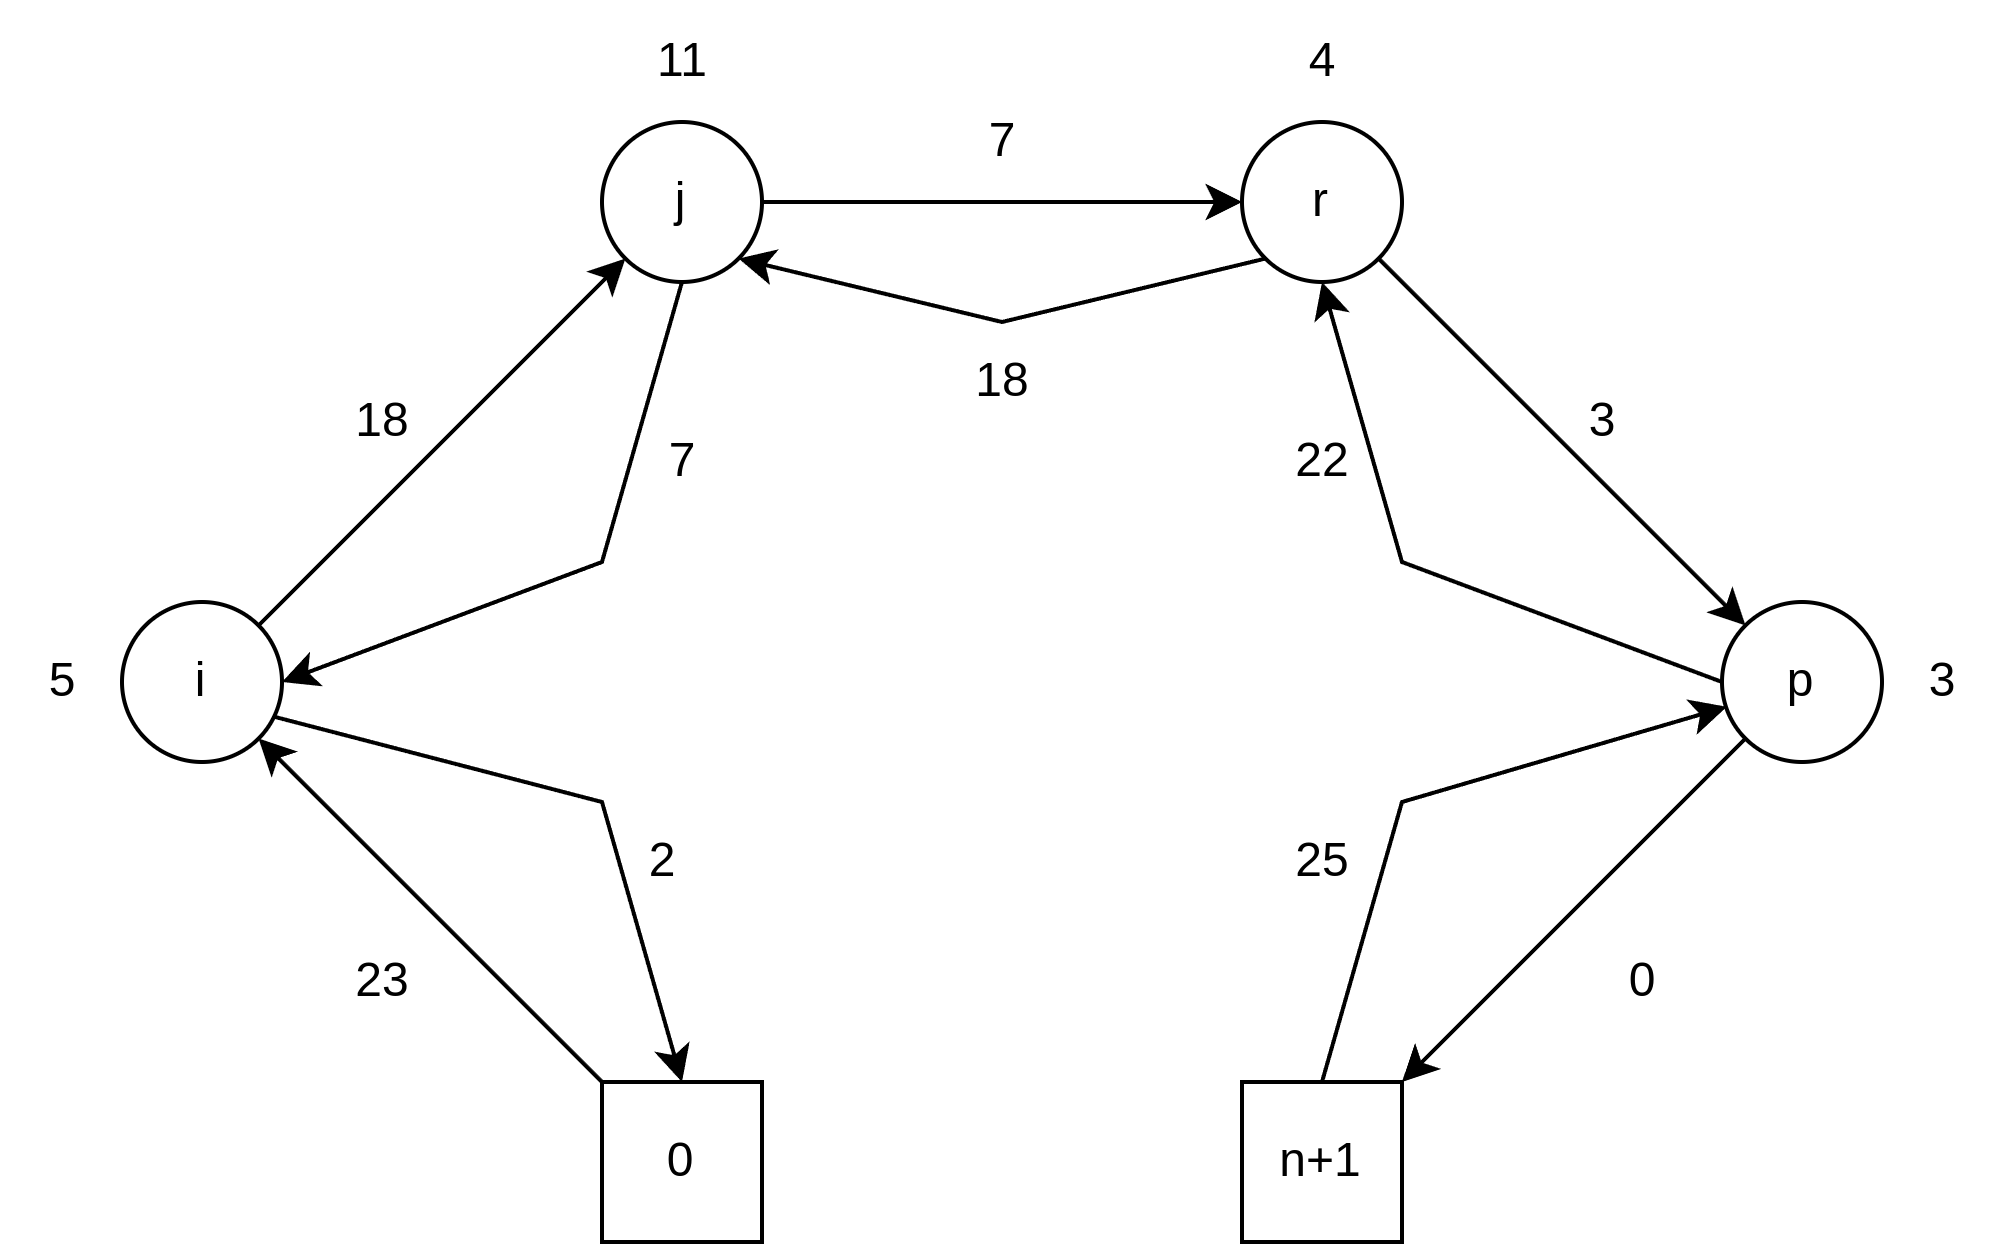
\includegraphics[width=0.8\textwidth]{figures/commondity-flow-model.png} 
  % \includesvg[scale=1]{figures/core-object}
  \caption{Minh họa dòng hàng với $Q=25$} 
  % \label{fig:fg_02}
\end{figure}

\subsection{Công thức phân hoạch tập hợp và thuật toán}
Công thức phân hoạch tập hợp đơn giản của VRP lần đầu được nghiên cứu bởi Balinski, Quandt (1964) \cite{balinski1964integer}. Gọi $r$ là một tuyến, $a_{ir}$ là hệ số nhị phân có giá trị bằng $1$ khi và chỉ khi nút $i \in V \setminus \{0\}$ thuộc tuyến $r$, gọi $c^*$ là chi phí tối ưu của tuyến $r$ và gọi $y_k$ la biến nhị phân bằng $1$ khi và chỉ khi tuyến $r$ được dùng trong lời giải tối ưu. Bài toán được mô hình hóa như sau

\begin{equation}
	\min \sum_r{c_r^* y_r}
\end{equation}
s.t.
\begin{flalign}
	\label{ct4:1} & \sum_r a_{ir} = 1 & \quad (i \in V \setminus \{0\}), \\
	\label{ct4:2} & \sum_r y_r = m,   & \quad                            \\
	\label{ct4:3} & y_r = 0, 1        & \quad (\text{mọi } r).
\end{flalign}

Nói một cách chặt chẽ thì ràng buộc (\ref{ct4:2}) không phải một phần của công thức phân hoạch tập hợp chuẩn, tuy nhiên nó được sử dụng bởi hầu hết các nhà nghiên cứu trong trường hợp VRP.

\section{Heuristics cổ điển}

Nhìn chung thì các thuật toán giải chính xác khó đảm bảo hiệu năng trong thực tế khi mà các tập dữ liệu ngày các lớn và các doanh nghiệp cần phục vụ khách hàng một cách nhanh chóng và tiết kiệm. Thực tế người ta cần tìm ra một (số) lời giải chập nhận được đủ tốt trong một khoảng thời gian "hợp lý". Từ những năm 1964 cho đến 1990, rất nhiều heuristics được nghiên cứu. Một số ít là đưa ra thuật toán hoàn toàn mới còn hầu hết là cải tiến thuật toán đã có.

\subsection{Thuật toán tiết kiệm}

Thuật toán tiết kiệm được đưa ra bởi Clark, Wright (1964) \cite{clarke1964scheduling}, mô tả và cài đặt khá đơn giản nhưng vẫn đưa ra được nghiệm tốt. Chính vì thế, thuật toán này được sử dụng rất rộng rãi. Thuật toán bắt đầu với nghiệm ban đầu với $n$ tuyến $(0, i, 0)$ với $i \in V \setminus \{0\}$. Tại mỗi vòng lặp thuật toán nối tuyến kết thúc với $i$ với một tuyến khác bắt đầu với $j$ cực đại hóa đại lượng \textit{tiết kiệm} $s_{ij}=c_{i0} + c_{0j} - c_{ij}$ và lới giải mới thỏa mãn các ràng buộc. Quá trình kết thúc khi không thể nối các tuyến vào nữa.

Một số cải tiến được đề xuất, ví dụ như nhân $c_{ij}$ với một trọng số dương $\lambda$ (Golden, Magnanti, Nguyen (1977) \cite{golden1977implementing}), tối ưu tuyến đường hợp nhất toàn cục thông qua việc sử dụng thuật toán phù hợp (Altinkemer, Gavish (1991) \cite{altinkemer1991parallel} và Wark, Holt (1994) \cite{wark1994repeated}), tăng tốc tính toán (Paessens (1988) \cite{paessens1988savings})...

\subsection{Phân cụm trước, định tuyến sau}

Heuristic phân cụm trước, định tuyến sau của Fisher, Jaikumar (1981) \cite{fisher1981generalized} trước hết đặt $m$ tâm và phân cụm sao cho tổng khoảng cách từ các nút đến tâm của nó là nhỏ nhất và thỏa mãn về ràng buộc tải trọng. Sau đó trên mỗi cụm, tuyến đường được thiết lập bằng cách giải bài toán TSP. Một vài chiến thuật để khởi tạo cũng như lựa chọn tâm cụm được trình bày trong Baker, Sheasby (1999) \cite{baker1999extensions}

\subsection{Heuristics cải tiến}

\section{Metaheuristics}

Metaheuristics có thể được phân lọai thành tìm kiếm lân cận, tìm kiếm phổ biến và cơ chế học. Hầu hết các thuật toán metaheuristics cho VRP đều dựa trên tìm kiếm lân cận và là các phương pháp cải tiến. Các thuật toán tốt nhất khá mạnh mẽ ngay cả khi nghiệm khởi tạo có chất lượng thấp. Một xu hướng chung là thay vì sử dụng chỉ một thuật toán, người ta thường kết hợp nhiều thuật toán lại với nhau. Các thuật toán như vậy được gọi là thuật toán lai.

Tiếp theo tác giả trình bày ý tưởng chính của một số lớp thuật toán metaheurictics.

\subsection{Tìm kiếm cục bộ}

Về cơ bản, tìm kiếm lân cận cố gắng "khám phá" không gian nghiệm bằng cách "di chuyển" quanh nghiệm hiện tại tới một nghiệm khác trong vùng lần cận của nó. Một số phương pháp có thể kể đến như \textit{tabu search} (Glover (1986) \cite{glover1986future}), \textit{simulated annealing} (Kirkpatrick, Gelatt, and Vecchi
(1983) \cite{kirkpatrick1983optimization}), \textit{deterministic annealing} (Dueck, Scheurer
(1990) \cite{dueck1990threshold}; Dueck (1993) \cite{dueck1993new}), \textit{variable neighbourhood search} (Mladenović, Hansen (1997) \cite{mladenovic1997variable}), \textit{large neighbourhood search}(Shaw (1998) \cite{shaw1998using}) và \textit{adaptive large neighbourhood search} (Ropke, Pisinger (2006) \cite{ropke2006adaptive}). Các thành phần chính của tìm kiếm lân cận là các quy tắc để xác định vùng lân cận của một nghiệm và cơ chế để khám phá vùng lân cận đó.

Trong \textit{tabu search} không gian nghiệm được khám phá bằng cách di chuyển từ nghiệm hiện tại đến nghiệm tốt nhất trong một tập con của lân cận của nghiệm đó. Để tránh việc lặp lại các nghiệm, các nghiệm được gán một thuộc tính gắn với nghiệm hiện tại để không được chọn trong một số lần lặp tiếp theo. Một nghiệm trở thành nghiệm tốt nhất trong số các nghiệm đã biết có thuộc tính gắn với thuộc tính hiện tại. Nguyên lý này được trình bày đầu tiên bởi Cordeau, Gendreau, Laporte (1997) \cite{cordeau1997tabu} và hiện nay được biết đến như là phương pháp tìm kiếm dựa trên thuộc tính (Derigs, Kaiser (2007) \cite{derigs2007applying}).

Trong \textit{simulated annealing} một gnhiệm $x$ được chọn ngẫu nhiên trong lân cận $N(x_t)$ của nghiệm hiện tại $x_t$ tại vòng lặp $t$. Nếu hàm mục tiêu $f$ cực tiểu, ta gán $x_{t+1}:=x$ với $f(x_{t+1}) \leq f(x_t)$. Ngược lại gán $x_{t+1}:=x$ với một xác suất $p_t$ và gán $x_{t+1}:=x_t$ với xác suất $1-p_t$. Trong đó, $p_t$ là một hàm giảm theo $t$ và $f(x) - f(x_t)$.

Trong \textit{deterministic annealing}, nghiệm $x$ cũng được chọn ngẫu nhiên trong lân cận $N(x_t)$. Trong thuật toán \textit{threshold-accepting} (Dueck, Scheurer (1990) \cite{dueck1990threshold}), $x_{t+1}:=x$ khi $f(x) < f(x_t) + \theta_1$, với $\theta_1$ là một trọng số dương; ngược lại gán $x_{t+1}:=x_t$. Trong \textit{record-to-record travel} (Dueck (1993) \cite{dueck1993new}), với nghiệm tốt nhất hiện tại $x^*$, gán $x_{t+1}:=x$ nếu $f(x) \leq \theta_2 f(x^*)$, với $\theta_2$ là một trọng số dương; ngược lại gán $x_{t+1}:=x_t$.; ngược lại gán $x_{t+1}=x_t$.

Trong \textit{Variable neighbourhood search} (Mladenović, Hansen (1997) \cite{}), tác giả xem xét một dánh sách được sắp xếp của các lân cận. Thuật toán bắt đầu với một lân cận và chuyển qua lân cận tiếp theo cho đến khi đạt tới nghiệm tối ưu cục bộ. Việc tìm kiếm được khởi tạo lại khi một nghiệm tốt hơn được tìm thấy hoặc tất cả các lân cận đã dược xét qua. \textit{Very large-scale neighbourhood search - LNS} bỏ đi và tạo lại một (vài) phần của nghiệm hiện tại để tìm kiếm nghiệm tốt hơn. Nguyên lí này giống như cơ chế hủy và tạo lại được trình bày bởi Shaw (1998) \cite{shaw1998using}. \textit{Adaptive large neighbourhood search - ALNS} (Ropke, Pisinger (2006) \cite{ropke2006adaptive}) được biết đến như là một phiên bản mạnh mẽ hơn của \textit{large neighbourhood search}, trong đó các thuật toán hủy hay tạo lại được lựa chọn một cách linh hoạt và thích ứng với trạng thái hiện tại của hệ. LNS và ALNS là cảm hứng chính cho luận văn này. Trong các phần tiếp theo tác giả sẽ trình bày chi tiết về ALNS.

\subsection{Tìm kiếm quần thể}

Tìm kiếm quần thể hoạt động với một quần thể các nghiệm. Thuật toán di truyền (Holland (1975) \cite{holland1975adaptation}) là ví dụ tốt nhất cho mô hình này. Tại mỗi vòng lặp, một vài nghiệm cha dược trích xuất từ quần thể hiện tại và kết hợp để tạo ra các nghiệm con. Nghiệm con sau đó được thay bằng những phần tệ nhất trong quần thể nếu điều này cải thiện nghiệm tốt nhất hiện tại. Về cơ bản, thuật toán áp dụng đa dạng hóa các cơ chế, gọi là đột biến cho thế hệ nghiệm con trước khi xem xét việc đưa chúng vào quần thể.


\subsection{Cơ chế học}

Cơ chế học vay mượn ý tưởng từ trí tuệ nhân tạo với mạng thần kinh (neural networks). Thuật toán học hỏi kinh nghiệm và điều chỉnh các trọng số qua các vòng lặp. Ứng dụng với VRP được trình bày bởi Ghaziri (1991) \cite{ghaziri1991solving}; Schumann, Retzko (1995) \cite{schumann1995self}. Thuật toán tối ưu đàn kiến cũng là một dạng khác của cơ chế học. Nó bắt chước hành vi của đàn kiến trong việc tìm thức ăn và để lại vết trên đường đi. Theo thời gian, vết được để lại nhiều hơn trên đường đi ngắn nhất và qua đó, kiến đi theo con đường này. Ứng dụng đầy đủ được trình bày bởi Reimann, Doerner, Hartl (2004) \cite{reimann2004d}



    \end{content}
    
    \pagenumbering{Roman}
    \setcounter{page}{\numexpr\value{savepage}}

    % References
    \references{}

    
    % Appendix
    %  \begin{appendix}
    %     % In the appendices, use \section{} instead of \chapter{}
    %      \section{Some Appendix Section}
\label{sec:appendix01}
Appendices provide only two structural levels, viz., \texttt{\textbackslash section}, and \texttt{\textbackslash subsection}.

The numbering of figures, listings, tables, and footnotes is not reset. Thus, it continues as usual in the appendix.

\subsection{Some Appendix Subsection}

\lipsum[10]
    %  \end{appendix}




    % Declaration of authorship
    % \authorshipstatement[pagenumbering=false]
    % \authorshipstatement[pagenumbering=true]
    % \authorshipstatement[pagenumbering=only]
    
    % Consent form for use of plagiarism detection software
    % Not yet required
    % \consentform[pagenumbering=false]
    % \consentform[pagenumbering=true]
    % \consentform[pagenumbering=only]
    
    % Bonus: Wordcount
    % cd %FOLDER WHERE THE .tex FILES ARE IN %
    % clear
    % texcount -total -q -col -sum *.tex
    
\end{document}
